% REMEMBER TO SET LANGUAGE!
\documentclass[a4paper,10pt,english]{article}
\usepackage[utf8]{inputenc}
\usepackage[english]{babel}
\usepackage[titletoc]{appendix}
% Standard stuff
\usepackage{amsmath,graphicx,babel,varioref,verbatim,amsfonts}
% colors in text
\usepackage[usenames,dvipsnames,svgnames,table]{xcolor}
% Hyper refs
\usepackage[framestyle=none,framefit=yes,heightadjust=all,framearound=all]{floatrow}    
\floatsetup[figure]{style=Boxed,framearound=all}
\usepackage{fancyhdr}
\usepackage[colorlinks]{hyperref}

% Document formatting
\setlength{\parindent}{0mm}
\setlength{\parskip}{1.5mm}
%\setcounter{section}{-1} Hvis du vil ha 0 som første avsnitt
\numberwithin{figure}{subsection} 
\numberwithin{table}{subsection}
\numberwithin{equation}{subsection}

%Color scheme for listings
\usepackage{textcomp}
\definecolor{listinggray}{gray}{0.9}
\definecolor{lbcolor}{rgb}{0.9,0.9,0.9}

%Listings configuration
\usepackage{listings}
\lstset{
	backgroundcolor=\color{lbcolor},
	tabsize=4,
	rulecolor=,
	language=c++,
        basicstyle=\scriptsize,
        upquote=true,
        aboveskip={1.5\baselineskip},
        columns=fixed,
	numbers=left,
        showstringspaces=false,
        extendedchars=true,
        breaklines=true,
        prebreak = \raisebox{0ex}[0ex][0ex]{\ensuremath{\hookleftarrow}},
        frame=single,
        showtabs=false,
        showspaces=false,
        showstringspaces=false,
        identifierstyle=\ttfamily,
        keywordstyle=\color[rgb]{0,0,1},
        commentstyle=\color[rgb]{0.133,0.545,0.133},
        stringstyle=\color[rgb]{0.627,0.126,0.941}
        }
        
%User settings
\newcommand{\eqs}{\begin{equation}}
\newcommand{\eqf}{\end{equation}}
\newcounter{subproject}
\renewcommand{\thesubproject}{\alph{subproject}}
\newenvironment{subproj}{
\begin{description}
\item[\refstepcounter{subproject}(\thesubproject)]
}{\end{description}}
\newcommand{\HRule}{\rule{\linewidth}{0.5mm}}

%Other
\usepackage{geometry}
\usepackage{booktabs}
\newcommand{\shaderow}{\rowcolor{gray!20}[2pt][2pt]}
\usepackage[boxed,linesnumbered,lined]{algorithm2e}

%Lettering instead of numbering in different layers
%\renewcommand{\labelenumi}{\alph{enumi}}
%\renewcommand{\thesubsection}{\alph{subsection}}

\title{Project 2 - FYS3150}
\author{Vidar Skogvoll}


\begin{document}
%Header
\pagestyle{fancy}
\renewcommand{\sectionmark}[1]{\markright{#1}{}}

\pagestyle{fancy}
\renewcommand{\sectionmark}[1]{\markright{\thesection\ #1}}

\fancyhf{}
%Header
%\rhead{\fancyplain{}{ NAVN PÅ PROSJEKT}} % predefined ()
\lhead{\fancyplain{}{\rightmark }} % 1. sectionname, 1.1 subsection name etc
\cfoot{\fancyplain{}{\thepage}}

\maketitle

\newpage
\hypersetup{linkcolor=black}
\tableofcontents
\hypersetup{linkcolor=red}
\newpage 


\section{Introduction}

Quantum theory is often thougth of as 
"the most precisely tested and most successful theory in the history of science" 
\footnote{\url{http://www.4physics.com/phy_demo/QM_Article/article.html}}, 
which is not a controversial statement. 
But the despite the success of the theory, the mathematical foundation upon which it is built is 
more or less the same as it was 50 years ago. 
However, the computational power available has grown exponatially the last 30 years, 
allowing us to explore the mysteries of quantum systems within a couple of minutes of 
computational time. 
The motivation for this project is to explore one such quantum system by approximating it 
to a linear algebra eigenvalue problem and look at the properties of such an approximation. 

In this project I have written a class in c++-language in which I can enter the properties 
of the discretization of a system with a
particle in a spherical symmetric potential and and find the energy eigenstates of the system. 
The concrete systems to which this class has been applied are described in the theory section
(sections \ref{sec:systems})
I have programmed the Jacobi algorithm (described in section \ref{sec:jacobi}) to
solve the eigenvalue problem of the class.

The systems are discretized and so we might expect some deviation from what is the 
exact solutions of the systems.
That is why I have also investigated the precision of the methods as functions 
of the discretization limits. 
Another aspect of the algorithm used is the efficacy of it, and how much time it uses 
to perform a specific task when compared to other methods. 
This has also been investigated. 

When solving the exercise I noticed some strange properties of the discretization
which I have done some preliminary investigation on as a final remark 
and possible continnuation project. 
One example of such a property is that the eigenvalue solver seems to return 
the very first (as in lowest energy) eigenstates. 
Why is this? 
If we include a potential in which we have degenerate energies, will this phenomenon still occur?




























\section{Theory}\label{sec:theory}

\subsection{The physical quantum system}\label{sec:systems}

The bound energy states of the hamiltonian are composed of two parts. 
The spherical harmincal functions and what we will describe as the \textit{radial part} $R(r)$. 
It can be shown, using separation of variables that the radial part must satisfy the equation below

\eqs -\frac{\hbar^2}{2 m} \left ( \frac{1}{r^2} \frac{d}{dr} r^2
  \frac{d}{dr} - \frac{l (l + 1)}{r^2} \right )R(r) 
     + V(r) R(r) = E R(r) \eqf

Now introducing new variables $u(r) = r R(r)$ and $\rho = r/\alpha$ it 
is possible to rewrite the equation above as 

\eqs 
 -\frac{d^2}{d\rho^2} u(\rho) + V (\rho)
 u(\rho)  = \lambda u(\rho)
 \eqf 
For some clever choice of the constants $\alpha$ and $\lambda$ dependent on the 
potential
where $V$ is the effective potential defined as 

\eqs V(\rho) = V_0(\rho) + \frac{l(l+1)}{\rho^2} \label{eq:TUSL} \eqf

and $V_0(\rho)$ is the real potential of $\rho$.
It is equation \ref{eq:TUSL} this project is trying to solve for different potentials.

\subsubsection{Discretization and linear algebra}

We may discretize, for $i=0,1,2,...,n_{step}$, 
$u \rightarrow u_i$, $\rho \rightarrow \rho_i$ and $V(\rho) \rightarrow V_i$
 and use the standard expression for the second derivative
of a function $u$.

\eqs u''=\frac{u(\rho+h) -2u(\rho) +u(\rho-h)}{h^2} +O(h^2),
    \label{eq:diffoperation} \eqf

where $h$ is our step length.
Introducing the boundary conditions that $u(0) = 0$ and $u(\rho_{max}) = 0$ 
lets us transform
(as shown in project 1)
equation \ref{eq:TUSL} into the linear algebra problem given by equation \ref{eq:linalg}.

\eqs
\begin{matrix}
 \left( \begin{array}{ccccccc} \frac{2}{h^2}+V_1 & -\frac{1}{h^2} & 0   & 0    & \dots  &0     & 0 \\
                                -\frac{1}{h^2} & \frac{2}{h^2}+V_2 & -\frac{1}{h^2} & 0    & \dots  &0     &0 \\
                                0   & -\frac{1}{h^2} & \frac{2}{h^2}+V_3 & -\frac{1}{h^2}  &0       &\dots & 0\\
                                \dots  & \dots & \dots & \dots  &\dots      &\dots & \dots\\
                                0   & \dots & \dots & \dots  &\dots       &\frac{2}{h^2}+V_{n_{\mathrm{step}}-2} & -\frac{1}{h^2}\\
                                0   & \dots & \dots & \dots  &\dots       &-\frac{1}{h^2} & \frac{2}{h^2}+V_{n_{\mathrm{step}}-1}

             \end{array} \right)  

\left( \begin{array}{c} u_{1} \\
                                                              u_{2} \\
                                                              \dots\\ \dots\\ \dots\\
                                                              u_{n_{\mathrm{step}}-1}
             \end{array} \right) \\ \\ =\lambda \left( \begin{array}{c} u_{1} \\
                                                              u_{2} \\
                                                              \dots\\ \dots\\ \dots\\
                                                              u_{n_{\mathrm{step}}-1}
             \end{array} \right) \\ \end{matrix}        
\label{eq:linalg}
\eqf

Which is nothing but an eigenvalue problem which we will use Jacobi's method to solve
(see section \ref{sec:jacobi}).

\subsubsection{One particle in a harmonic oscillator}

For a particle in a three dimensional harmonic oscillator, the potential is given as 

\eqs V_0(r) = \frac{1}{2} m \omega^2 r^2 \eqf

The smart choice of $\alpha$ and $\lambda$ (as discussed in \ref{sec:systems}in this case is 

\eqs \alpha = \left ( \frac{\hbar}{m\omega} \right )^{1/2} \eqf

And 

\eqs \lambda = \frac{2m\alpha^2}{\hbar^2} \eqf

Because with these definition, the effective potential becomes 

\eqs V(\rho) = \rho^2 + \frac{l(l+1)}{\rho^2} \eqf

This effective potential will from here on be known as the 
"plain\_harmonic" potential.
It can be shown theoretically that this potential has eigenvalues $\lambda$ 
equal to 

\eqs
\lambda = 3 + 3n + 2l 
\label{eq:eig}
\eqf

For $n=0,1,2,...$ and $l = 0,1,...,n-1$. 
We will use this exact result as a measure of the error in the discretization of the 
problem. 








\subsubsection{Two electrons in a harmonic oscillator}\label{sec:theo2elec}

To simplify the problem we will now ignore the angular momentum quantum number $l$.
The general equation for two electrons with center of mass position $\vec R$ given by

\eqs \vec R = \frac{\vec r_1 + \vec r_2}{2} \eqf

And relative position $\vec r$ (i.e. position of the one with regards to the other) given by

\eqs \vec r = \vec r_1 - \vec r_2 \eqf

Where $\vec r_1$ and $\vec r_2$ are the positions operators for each of the electrons can be shown 
to be (see section \ref{sec:2elec} in the appendix)

\eqs \left(  -\frac{\hbar^2}{m} \frac{d^2}{dr^2} -\frac{\hbar^2}{4 m} \frac{d^2}{dR^2}+ \frac{1}{4} k r^2+  kR^2\right)u(r,R)  = E^{(2)} u(r,R).
\eqf

Now, using separation of variables, 
and adding the repulsive potential between the electrons 
, it is possible to show that the relative distance
wave function $\psi(\rho)$ of the two electrons must satisfy the following equation

\eqs
-\frac{d^2}{d\rho^2} \psi(\rho) + V(\rho) \psi(\rho) = \lambda \psi(\rho)
\eqf

Where $\rho = r/\alpha$ as before and $V(\rho)$ is the effective potential defined as 

\eqs V(\rho) = \omega_r^2\rho^2 + \frac{1}{\rho}  
\label{eq:two_elec_potential} \eqf

Where the three terms on the left hand side stems from the oscillator potential and 
the repulsive coulomb potential  respectively. 
The smart choices of $\alpha$, $\lambda$ and $\omega_r$ to obtain the equation above are as follows

\eqs \alpha = \frac{\hbar^2}{m\beta e^2} \eqf
\eqs \lambda = \frac{m \alpha^2}{\hbar^2} E \eqf
\eqs \omega_r^2 = \frac{1}{4} \frac{mk}{\hbar^2} \alpha^4 \eqf

Where $\beta e^2 = 1.44 eV~ nm$. 
$\omega_r$ is a constant characterizing the strength of the harmonic oscillator. 
As we see, this is just a modification of the one dimensional problem discussed earlier
with a different potential, 
and we can use the eigenvalue solving mechanism to solve it.
The potential 

\begin{equation}
\omega_r^2\rho^2 + \frac{1}{\rho} \tag{\ref{eq:two_elec_potential}} 
\end{equation}

Will from here on be known as the "two\_elec" potential. 

\subsection{The jacobi rotation algorithm}\label{sec:jacobi}

Suppose we have a linear algebra eigenvalue problem

\eqs A\vec x = \lambda \vec x \eqf

and some simularity transformation such that 

\eqs S^T A S = D \eqf

Where $S$ is a unitary matrix and $D$ is a diagonal matrix. 
Linear algebra tells us that if $A$ is real and symmetric, there is always such a matrix 
and the Jacobi rotation algorithm finds us one. 
The method is explained at lengths in the lecture notes of the course \cite{lecturenotes}, 
but for this section's purpose, it suffices to say that the algorithm provides 
a set of unitary matrices $S_0,S_1,...,S_N$
so that 

\eqs A_N = S^T A S = S_N^T ... S_1^T A_0 S_1 ... S_N = D \eqf

At each iteration we save the matrix $A_i$ we get from calculation $A_i = S_i^T A_{i-1} S$.
Now, let's look at the eigenvalue problem with variable notation familiar with quantum mechanics. 

\eqs H \psi = E \psi \eqf

Here, $H$ is a real, symmetric matrix, $\psi$ is a eigenvector and $E$ is a eigenvalue. 
Applying $S^T$ from the left hand side 

\eqs S^T H \psi = E S^T \psi \eqf

Since $S$ is a unitary matrix we get

\eqs S^T H S S^T \psi = E S^T \psi \eqf
\eqs D S^T \psi = E S^T \psi  \label{eq:tmp2}\eqf

As we see, the eigenvalues $E$ of the diagonal matrix are the same as the eigenvalues of 
the initial matrix $A$. 
But since $D$ is diagonal we can just read the eigenvalues off of it.
The eigenvectors of the diagonal matrix are given by the identity matrix, but 
are also given as we see from equation \ref{eq:tmp2} as $S^T \psi$
(if $\psi$ is a matrix with eigenvector colums)
, thus

\eqs S^T \psi = I \eqf
\eqs S S^T \psi = S I \eqf
\eqs \psi = S \eqf

At each iteration we may save the matrix $V_i = S_i^T V_{i-1}$ where $V_0 = I$ and get 

\eqs V = S_N^T S_{N-1}^T ... S_1^T \eqf

If we transpose this matrix we get


\eqs V^T  = S_1 S_2 ... S_N = \psi \eqf

And then we know how to extract the eigenvectors, as well as the eigenvalues, 
from the algorithm.  
Since unitary matrices are norm preserving 
\footnote{Source: \url{http://en.wikipedia.org/wiki/Unitary_matrix}}
and $I$ is (obviously) an orthonormal matrix, 
the matrix $V^T$ will also be orthonormal which ensures that the states we 
get from this method are normalized. 

The $S$ matrices are known as jacobi rotation matrices and each similarity transformation is known 
as a rotation. 
Within the algorithm for the jacobi method there is a tolerance $\epsilon$ involved 
which lets us know when to stop the algortihm from running, i.e.
when we think our diagonal matrix is "diagonal enough". 
The algorithm stops when the largest off-diagonal element $m$ squared is bigger than 
the given tolerance, in other words, when $m^2 > eps$. 
Througout this project, $\epsilon = 10^{-10}$. 

































\section{Method}

\subsection{The error in the eigenvalues as a function of $n_{step}$ and $\rho_{max}$}
\label{sec:error_nstep_rhomax}
In reality, the coordinate $\rho$ can take any value between $0$ and $\infty$. 
This is, for obvious reasons, not a possibility when discretizing and 
using nummerical methods. 
Therefore we must explicitly set the value of $\rho_{max}$ at which point the 
wave function should be zero.

This is an approximation. 
So is the number $n_{step}$ of discretization steps we take, and so 
this part will deal with the error in the eigenvalues of the "plain\_harmonic" potential
(given by equation \ref{eq:eig}) 
as a function of $n_{step}$ and $\rho_{max}$. 

The script \textbf{error\_nstep\_rhomax.cpp} 
(see section \ref{sec:error_nstep_rhomax.cpp})
investigated the error in the obtained eigenvalues as a function of different 
$n_{steps}$ and $\rho_{max}$. 
$l$ was set to equal $0$ for simplicity. 




\subsection{Number of rotations as a function of dimensionality}

The number of rotations needed in the Jacobi algorithm to meet the required tolerance is 
expected to increase as a function of the dimensionality, i.e. the discretization resolution. 

The script \textbf{number\_rotations\_dim.cpp} (see section \ref{sec:number_rotations_dim.cpp})
investigated number of rotations needed as a function of dimensionality $n_{step}$
with a "plain\_harmonic"-potential with $l=0$.


\subsection{Timely difference between jacobi algorithm and another algorithm}

Another interesting aspect of this problem is to compare the execution time of
the jacobi algorithm with another algorithm. 

The script \textbf{compare\_times\_arma\_jacobi.cpp} 
(see section \ref{sec:compare_times_arma_jacobi.cpp}) 
investigated the time used to solve the problem with $\rho_{max} = 6$ and
the 
"plain\_harmonic"-potential with $l=0$
for different values of $n_{step}$. 
And compared the elapsed time from the jacobi algorithm to that of the 
algorithm named "eig\_sym" provided by the armadillo library. 

\subsection{Degeneration with $l \neq 0$}

In a real system with a three dimensional harmonic oscillator,
there is, for $l\neq 0$ a degeneracy of the energies. 
This because there are two quantum numbers, $l$ and $m$, 
involved in the spherical harmonical functions and for each $l$ 
$m$ can take values $m= -l, -l+1 , ... , l-1, l$,
while the energy, as we may read from equation \ref{eq:eig}, 
is not dependent on $m$. 
An interesting question is whether we will see this degeneration when 
computing the eigenenergies of our system or not. 

The script \textbf{degeneration.cpp} (see section \ref{sec:degeneration.cpp}) 
investigated this issue.


\subsection{The two-electron system}

We will now look at some of the specifics of the two-electron system with 
the repulsive potential as described in section \ref{sec:theo2elec}. 

The script \textbf{two\_electrons.cpp} (see section \ref{sec:two_electrons.cpp})
solved problem of the relative distance between the two electrons 
for three different values of $\omega_r$ 
(three different harmonical potential strengths). 





























\newpage
\section{Results and discussion}

\subsection{The error in the eigenvalues as a function of $n_{step}$ and $\rho_{max}$}
Figure \ref{fig:error_nstep_rhomax} shows the results from running the script 
described in section \ref{sec:error_nstep_rhomax}.

\begin{figure}[h!]
  \centering
  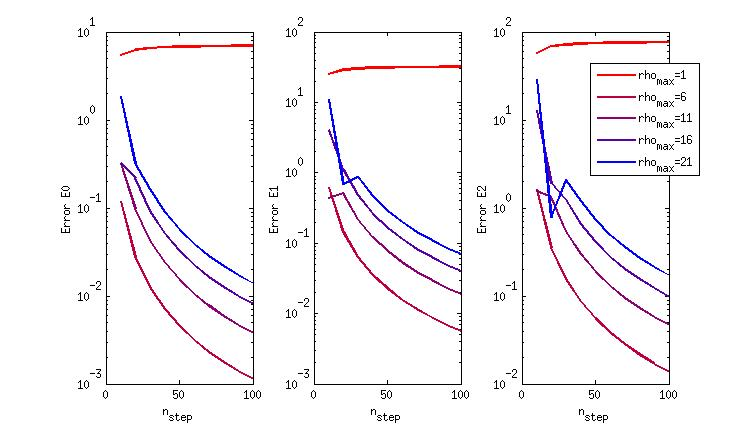
\includegraphics[width=\textwidth]{error_nstep_rhomax.jpg}
  \caption{Semilogaritmic plot of the absolute error in the 
    estimation of the first three eigenvalues $E_0 = 3$, $E_0 = 7$ and $E_0 = 7$. 
    For $\rho_{max} \geq 6$ the precision increases as a function of the resolution 
    $n_{step}$ but decreases as a function of $\rho_{max}$.}
  \label{fig:error_nstep_rhomax}
\end{figure}

The figure shows several insteresting aspects. 
Firstly, it clearly demonstrates that for a too small value of $\rho_{max}$, 
in this case $\rho_{max}= 1$ the number $n_{steps}$ of discretization steps does not 
matter. 
The error is present and doesn't change considerably with increasing $n_{step}$
When the value of $\rho_{max}$ gets larger however, we see that 
the precision of the estimation gets better with increased number $n_{step}$ of 
discretization points,
which is what one would expect. 

Secondly, we see that the precision in the approximatiom of these first 
few eigenvalues decrease as $\rho_{max}$ increases. 
This is not surprising, seeing as the first few eigenfunctions
(to which these eigenvalues apply) 
decrease in magnitude when $\rho$ becomes larger. 
Having more points in the area where the eigenfunctions really matter, 
i.e. near $0$ - small $\rho_{max}$,
would naturally cause better estimations of the eigenvalues as well. 

Finally, we see that the error in general increases with which 
increasing eigenvalues. 
This is because the eigenfunctions become more complicated for 
the more excited states and more points are needed to represent them 
with the same precision. 



\subsection{Number of rotations as a function of dimensionality}

Figure \ref{fig:number_rotations_dim} shows the results from counting the number of rotations 
as a function of the matrix dimensionality $n_{step}$. 

\begin{figure}[h!]
  \centering 
  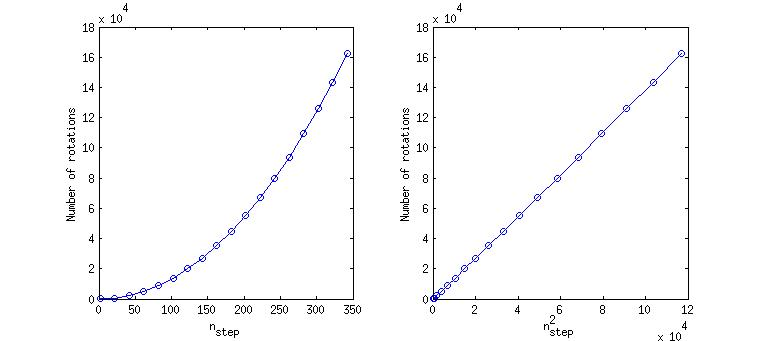
\includegraphics[width=\textwidth]{number_rotations_dim.jpg}
  \caption{Plot of the number of rotations (see section \ref{sec:jacobi}) used in the jacobi  
            algorithm against the
            dimensionality $n_{step}$ of the matrix. 
            The right hand plot shows a plot of the number of rotations as a function of 
            dimensionality $n_{step}$ of the matrix squared.
            The number of rotations increase with the dimensionality of matrix, 
            and there seems to be a quadratic trend.}
  \label{fig:number_rotations_dim}
\end{figure}

As expected, the number of rotations increases as a function of $n_{step}$. 
From the right hand side of the figure, it seems like a fair assumption that the number of 
rotations $Rot (n_{step})$ needed to obtained the wanted accuracy 
 is proportional to the dimensionality $n_{step}$ squared, i.e.

\eqs 
Rot(n_{step}) = k n_{step}^2 
\label{eq:rot_nstep}
\eqf

Where $k$ is some proportionality constant. 
An estimate of this constant based upon the data obtained is given in table \ref{tab:rot_nstep}.

\begin{table}[h!]
  \centering 
  \begin{tabular}{ll}
  \toprule
  What & Value \\
  \midrule
  k &  $ 1.376 \pm 0.006 $ \\
  \bottomrule
  \end{tabular}

  \caption{The estimation of the proportionality constant between jacobi rotations 
          and the dimensionality $n_{step}$ of the matrix squared (equation \ref{eq:rot_nstep}).
          The error estimation is made using MATLAB's curve fitting tool with a confidence interval 
          of $95\%$}
  \label{tab:rot_nstep}
\end{table}

The narrow confidence interval in the estimation of the proportionality constant $k$ 
confirms that the number of rotations $rot$ is indeed a quadratic function of 
the dimensionality $n_{step}$ of the matrix. 
This is also in agreement with the lecture notes 
which states that 
"one needs typicically $3n^2 - 5n^2$ rotations [...] to zero out the non-diagonal elements"
\footnote{Lecture notes \cite{lecturenotes}, p.217}.
The reason for this problem needing only $1.376 n^2$ rotation may be  
due to most off-diagonal elements being $0$ in the first place 
or that our tolerance for the largest off-diagonal element is 
high. 

An interesting question for another project would be to investigate how this
proportionality holds for other tolerances in the jacobi rotation algorithm. 
And if so, how the proportionality constant $k$ depends on the tolerance of the 
algorithm.


\subsection{Timely difference between jacobi algorithm and another algorithm}

The times needed to solve the problem with the different algorithms are
given in table \ref{tab:comparetimes}. 

\begin{table}[h!]
  \centering 
  \begin{tabular}{l @{ }  l @{  }l}
    \toprule
    Dimensionality $n_{step}~~$ & Jacobi algorithm time [s]$~~$& Armadillo algorithm time [s] \\
    \midrule
    10 & $9.4\times 10^{-5}$ & $3.0 \times 10^{-5}$ \\
    \shaderow 30 & $6.0 \times 10^{-3}$  &$2.4 \times 10^{-4}$  \\
    50 & $4.1\times 10^{-2}$ & $7.5\times 10^{-4}$ \\
    \shaderow 70 & $1.2 \times 10^{-1}$ & $1.5 \times 10^{-3}$ \\
    90 & $3.6 \times 10^{-1}$ & $2.6 \times 10^{-3}$ \\
    \shaderow 110 &$7.8 \times 10^{-1}$ & $4.1 \times 10^{-3}$ \\
    130 &$1.4 \times 10^{0}$ &  $6.2 \times 10^{-3}$\\
    \shaderow 150 &$2.7 \times 10^{0}$ &  $8.8 \times 10^{-3}$\\
    170 &$4.5 \times 10^{0}$ &  $1.2 \times 10^{-2}$\\
    \shaderow 190 &$7.0 \times 10^{0}$ &  $1.6 \times 10^{-2}$\\
    210 &$1.0 \times 10^{1}$ &  $2.1 \times 10^{-2}$ \\
    \bottomrule
  \end{tabular}
  \caption{The times needed to solve the eigenvalue problem using the jacobi- and the 
            armadillo algorithm as a function of the matrix dimensionality $n_{step}$. 
            Time elapsed increases with $n_{step}$ and it seems that the algorithm
            used by armadillo is much more efficient than the jacobi algorithm.}
  \label{tab:comparetimes}
\end{table}

A plot of the elapsed times from table \ref{tab:comparetimes} is given in figure
\ref{fig:comparetimes}. 

\begin{figure}[h!]
  \centering 
  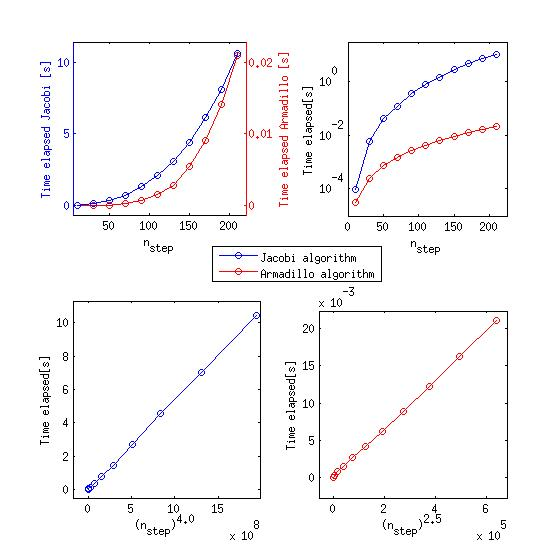
\includegraphics[width=\textwidth]{compare_times_arma_jacobi.jpg}
  \caption{Plot of the elapsed times from solving the eigenvalue problem with 
            different algorithms (see table \ref{tab:comparetimes})
            with different axes in different plots.
            We see that the algorithm used by the armadillo library is much more efficient 
            than the jacobi algorithm
            and that the they depend differently with respect to the 
            dimensionality $n_{step}$. }
  \label{fig:comparetimes}
\end{figure}

As we see from the results, the algorithm provided by the armadillo lbirary is much more 
efficient when it comes to time elapsed than the jacobi algorithm.
The time elapsed is many orders of magnitudes larger for the jacobi algorithm than the 
armadillo algorithm.

As we see, the time elapsed for the jacobi algorithm is apperantly proportional
to the dimensionality $n_{step}$ of the matrix to the fourth power. 
As we saw in the section above, the number of rotations needed for the algorithm to 
finish went as $n_{step}^2$. 
This indicates, given that there is a proportionality between flops and time elapsd, 
that the number of floating points operations for each rotation goes as $n_{step}^2$. 
This, however, is \textit{not} in agreement with the lecture notes which 
states that 
"each rotation requires $4n$ operations" 
\footnote{Lecture notes \cite{lecturenotes}, p.217}.
An interesting topic for another time would be to investigate where this 
discrepency between this theoretical number of flops and time elapsed arises.

The figure (\ref{fig:comparetimes}) also show that the time elapsed for the 
algorithm provided by armadillo goes pretty much as  $(n_{step})^{2.5}$.  


\subsection{Degeneration with $l \neq 0$}

Running the script and looking at the eigenvalues revealed that the degeneration 
was not caught by this method of solving the problem. 
This is not surprising;
The quantum number $m$ does not affect the radial part 
of the states,
so the radial parts for the different states corresponding to different values of $m$ 
are the same. 
Since we are solving an eigenvalue problem with a real symmetric matrix we are guarantied to 
find $n_{step}$ linearly independent eigenvectors (i.e. radial functions) and
thus we simply couldn't have found the degeneracy. 


\subsection{The two-electron system}

A plot of the results from running the script is shown in figure \ref{fig:two_electrons}.


\begin{figure}[h!]
  \centering
  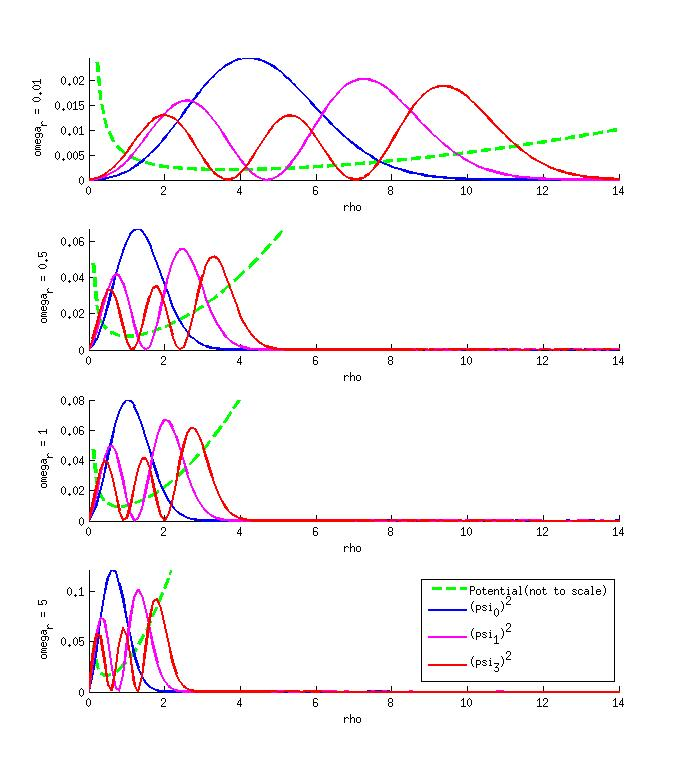
\includegraphics[width=\textwidth]{two_electrons.jpg}
  \caption{Plot of the probability density $\psi_i^2$ 
  as a function of the distance between the two electrons for 
  the three first eigenstates ($\psi_0$, $\psi_1$ and $\psi_2$)
  and four different 
  harmonic oscillator potential strengths (given by $\omega_r = 0.01, 0.5, 1 , 5$).
  We see that the electrons tend to be far apart for weaker harmonic oscillator potentials 
  and closer for the lowest energy states.}
  \label{fig:two_electrons}
\end{figure}

As we see from the figure the probability density of the distance between the electrons 
gets pressed towards $0$ as the potential "well" gets tighter, 
i.e. when the harmonic oscillator strengt $\omega_r$ gets bigger. 
This makes sense because a strong harmonic oscillator potential will 
draw the electrons very close together untill the repulsive coloumb force between them will 
equal the pull of the harmonic oscillator. 

We also see that the higher energy-states allows the electrons to be further apart. 
This is also natural since much energy is needed to be far apart in a potential "well".



















\clearpage
\section{Conclusion}



















\clearpage
\begin{appendices}
\HRule \\[0.4cm]
{ \huge \bfseries Appendix \\[0.4cm] }

\HRule \\[0.0cm]
\section{Deducing the equation for the two electron system.} \label{sec:2elec}

\textbf{The following reasoning has been shamelessly copy-pasted from the 
exercise instructions made by Morten Hjorth-Jensen, professor at UiO.}

We will now study two electrons in a harmonic oscillator well which
also interact via a repulsive Coulomb interaction.
Let us start with the single-electron equation written as
\[
  -\frac{\hbar^2}{2 m} \frac{d^2}{dr^2} u(r) 
       + \frac{1}{2}k r^2u(r)  = E^{(1)} u(r),
\]
where $E^{(1)}$ stands for the energy with one electron only.
For two electrons with no repulsive Coulomb interaction, we have the following 
Schr\"odinger equation
\[
\left(  -\frac{\hbar^2}{2 m} \frac{d^2}{dr_1^2} -\frac{\hbar^2}{2 m} \frac{d^2}{dr_2^2}+ \frac{1}{2}k r_1^2+ \frac{1}{2}k r_2^2\right)u(r_1,r_2)  = E^{(2)} u(r_1,r_2) .
\]


Note that we deal with a two-electron wave function $u(r_1,r_2)$ and 
two-electron energy $E^{(2)}$.

With no interaction this can be written out as the product of two
single-electron wave functions, that is we have a solution on closed form.

We introduce the relative coordinate ${\bf r} = {\bf r}_1-{\bf r}_2$
and the center-of-mass coordinate ${\bf R} = 1/2({\bf r}_1+{\bf r}_2)$.
With these new coordinates, the radial Schr\"odinger equation reads
\[
\left(  -\frac{\hbar^2}{m} \frac{d^2}{dr^2} -\frac{\hbar^2}{4 m} \frac{d^2}{dR^2}+ \frac{1}{4} k r^2+  kR^2\right)u(r,R)  = E^{(2)} u(r,R).
\]

\newpage
\section{Codes}
All the codes used in this project can also be found at 
\url{https://github.com/vidarsko/Project2}. 

\subsection{The library file}

\textbf{Header file: project2lib.h}
\lstinputlisting{project2lib.h}

\newpage
\textbf{Class file: project2lib.cpp}
\lstinputlisting{project2lib.cpp}

\newpage
\subsection{The error in the eigenvalues as a function of $n_{step}$ and $\rho_{max}$}
\label{sec:error_nstep_rhomax.cpp}
\textbf{error\_nstep\_rhomax.cpp}
\lstinputlisting{error_nstep_rhomax.cpp}

\newpage
\subsection{Number of rotations as a function of dimensionality}
\label{sec:number_rotations_dim.cpp}
\textbf{number\_rotations\_dim.cpp}
\lstinputlisting{number_rotations_dim.cpp}

\newpage
\subsection{Timely difference between the jacobi algorithm and another algorithm}
\label{sec:compare_times_arma_jacobi.cpp}
\textbf{compare\_times\_arma\_jacobi.cpp}
\lstinputlisting{compare_times_arma_jacobi.cpp}

\newpage
\subsection{Degeneration with $l\neq 0$}
\label{sec:degeneration.cpp}
\textbf{degeneration.cpp}
\lstinputlisting{degeneration.cpp}

\newpage
\subsection{The two-electron system}
\label{sec:two_electrons.cpp}
\textbf{two\_electrons.cpp}
\lstinputlisting{two_electrons.cpp}

\end{appendices}
\clearpage
\bibliography{bibliography}{}
\bibliographystyle{plain}
\end{document}
